%% LyX 2.2.2 created this file.  For more info, see http://www.lyx.org/.
%% Do not edit unless you really know what you are doing.
\documentclass[spanish]{article}
\usepackage[T1]{fontenc}
\usepackage[latin9]{inputenc}
\usepackage[paperwidth=19cm,paperheight=19cm]{geometry}
\usepackage{float}
\usepackage{booktabs}
\usepackage{graphicx}

\makeatletter

%%%%%%%%%%%%%%%%%%%%%%%%%%%%%% LyX specific LaTeX commands.
%% Because html converters don't know tabularnewline
\providecommand{\tabularnewline}{\\}

\makeatother

\usepackage{babel}
\addto\shorthandsspanish{\spanishdeactivate{~<>}}

\begin{document}

\section{Ejercicio 5}

Para la implementaci�n del sumador de 2 numeros en BCD de un digito
se observaron las diferencias entre la representaci�n binaria com�n
y la BCD para numeros del 0 al 19.

\begin{figure}[H]
\begin{centering}
\begin{tabular}{ccc}
\toprule 
Decimal & Binario & BCD\tabularnewline
\midrule
\midrule 
0 & 0000 0000 & 0000 0000\tabularnewline
\midrule 
1 & 0000 0001 & 0000 0001\tabularnewline
\midrule 
2 & 0000 0010 & 0000 0010\tabularnewline
\midrule 
3 & 0000 0011 & 0000 0011\tabularnewline
\midrule 
4 & 0000 0100 & 0000 0100\tabularnewline
\midrule 
5 & 0000 0101 & 0000 0101\tabularnewline
\midrule 
6 & 0000 0110 & 0000 0110\tabularnewline
\midrule 
7 & 0000 0111 & 0000 0111\tabularnewline
\midrule 
8 & 0000 1000 & 0000 1000\tabularnewline
\midrule 
9 & 0000 1001 & 0000 1001\tabularnewline
\midrule 
10 & 0000 1010 & 0001 0000\tabularnewline
\midrule 
11 & 0000 1011 & 0001 0001\tabularnewline
\midrule 
12 & 0000 1100 & 0001 0010\tabularnewline
\midrule 
13 & 0000 1101 & 0000 0011\tabularnewline
\midrule 
14 & 0000 1110 & 0001 0100\tabularnewline
\midrule 
15 & 0000 1111 & 0001 0101\tabularnewline
\midrule 
16 & 0001 0000 & 0001 0110\tabularnewline
\midrule 
17 & 0001 0001 & 0001 0111\tabularnewline
\midrule 
18 & 0001 0010 & 0001 1000\tabularnewline
\midrule 
19 & 0001 0011 & 00001 1001\tabularnewline
\bottomrule
\end{tabular}
\par\end{centering}
\caption{Comparativo Binario BCD}
\end{figure}
Se observ� un exeso de 6 para todos los numeros mayores a 9, es decir,
uno podria hacer la suma binaria y el resultado de 0 a 9 dar�a el
resultado esperado en BCD pero para resultados de 10 a 19 es necesario
un factor de correxi�n de +6. Para decidir si es mayor o menor a 9
se puede hacer un diagrama logico en el cual si hay carry en la suma
de los primeros cuatro bits, o esta encendido el MSB con el bit anterior,
o el MSB con el segundo se puede afirmar que es mayor a 9. Se esquematiz�
el siguiente bloque comparador:

\begin{figure}[H]
\begin{centering}
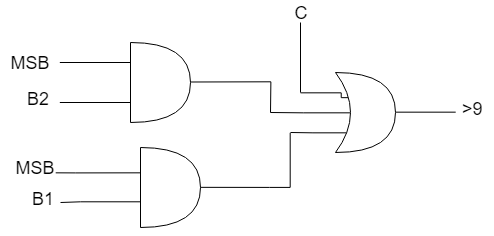
\includegraphics[scale=0.5]{ComparadorMayor9}
\par\end{centering}
\caption{Comparador mayor a 9}
\end{figure}

Se llevo a cabo el dise�o de un modulo ``Simple Adder'' el cual
deber�a poder hacer la suma con carry de 2 bits y devolver el resultado
y el carry de salida, para que luego bajo una conexi�n entre 4 de
estos podamos obtener la suma en binario de dos numeros de 4 bits
y un carry out de la suma total.

\begin{figure}
\begin{centering}
\begin{tabular}{ccccc}
\toprule 
a & b & Ci & Result & Co\tabularnewline
\midrule
\midrule 
0 & 0 & 0 & 0 & 0\tabularnewline
\midrule 
0 & 0 & 1 & 1 & 0\tabularnewline
\midrule 
0 & 1 & 0 & 1 & 0\tabularnewline
\midrule 
0 & 1 & 1 & 0 & 1\tabularnewline
\midrule 
1 & 0 & 0 & 1 & 0\tabularnewline
\midrule 
1 & 0 & 1 & 0 & 1\tabularnewline
\midrule 
1 & 1 & 0 & 0 & 1\tabularnewline
\midrule 
1 & 1 & 1 & 1 & 1\tabularnewline
\bottomrule
\end{tabular}
\par\end{centering}
\caption{Tabla Logica del Simple Adder}
\end{figure}

\begin{figure}
\begin{centering}
\begin{tabular}{|c|c|c|c|c|}
\hline 
\textbf{Ci\textbackslash{}ab} & \textbf{00} & \textbf{01} & \textbf{11} & \textbf{10}\tabularnewline
\hline 
\hline 
\textbf{0} & 0 & 1 & 0 & 1\tabularnewline
\hline 
\textbf{1} & 1 & 0 & 1 & 0\tabularnewline
\hline 
\end{tabular}
\par\end{centering}
\caption{Mapa de Karnau para Result}
\end{figure}

\begin{figure}
\begin{centering}
\begin{tabular}{|c|c|c|c|c|}
\hline 
\textbf{Ci\textbackslash{}ab} & \textbf{00} & \textbf{01} & \textbf{11} & \textbf{10}\tabularnewline
\hline 
\hline 
\textbf{0} & 0 & 0 & 1 & 0\tabularnewline
\hline 
\textbf{1} & 0 & 1 & 1 & 1\tabularnewline
\hline 
\end{tabular}
\par\end{centering}
\caption{Mapa de Karnau para Co}
\end{figure}

$Result=m_{1}+m_{2}+m_{4}+m_{7}=\bar{a}\bar{b}c+\overline{a}b\bar{c}+a\bar{b}\bar{c}+abc=\bar{a}(\bar{b}c+b\bar{c})+a(\bar{b}\bar{c}+bc)=\bar{a}(\bar{b}c+b\bar{c})+a\bar{(\bar{b}c+b\bar{c})}$,
recordando que $XOR=A\bar{B}+B\bar{A}$.

Calculo aux: $a(\bar{b}\bar{c}+bc)=\bar{\bar{a(\bar{b}\bar{c}+bc)}}=\bar{a+(\bar{\bar{b}\bar{c}+bc})}=\bar{a+(\bar{\bar{b}\bar{c}}\bar{bc})}=\bar{a+((b+c)(\bar{b}+\bar{c}))}=a\bar{(b\bar{c}+c\bar{b})}$.

$Co=Cib+Cia+ab=ab+Ci(a+b)$.

\begin{figure}[H]
\centering{}\includegraphics[scale=0.5]{\string"Modulo Simple Adder\string".png}\caption{Modulo Simple Adder}
\end{figure}

Habiendo dise�ado el m�dulo de Simple Adder se encadenaron 4 de estos
para formar efectivamente el modulo Bit4Adder donde obtenemos un resultado
final, un carry out y un overflow.

\begin{figure}[H]
\begin{centering}
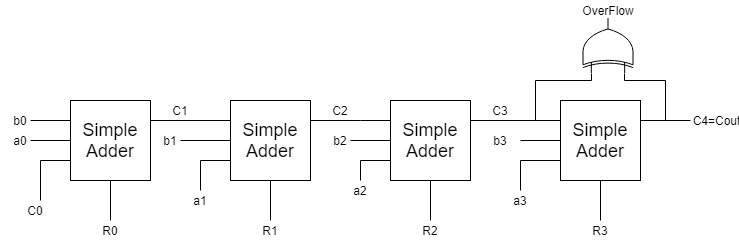
\includegraphics[scale=0.5]{Bit4Adderjpg}
\par\end{centering}
\caption{Bit4Adder}
\end{figure}

Con los m�dulos armados anteriormente podemos hacer nuestra suma BCD
donde nuestro comparador nos termina sumando 0110 a nuestra respuesta
de la suma original si excede 1001. De esta manera obtenemos un numero
de 8 bits representando hasta 19 en BCD.

\begin{figure}[H]
\begin{centering}
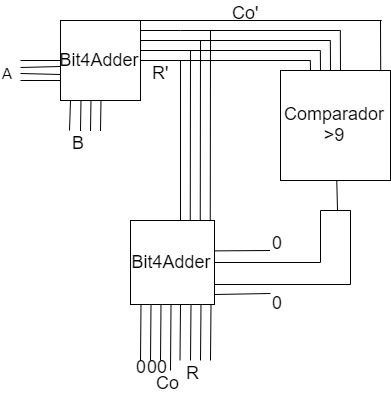
\includegraphics[scale=0.5]{SumaDeBCD}
\par\end{centering}
\caption{Bit4Adder}
\end{figure}


\section{ALU}

Para el dise�o de la ALU se reutilizaron los m�dulos vistos anteriormente
para hacer el complemento a 2 y la suma de 4 bits. 

\begin{figure}[H]
\begin{centering}
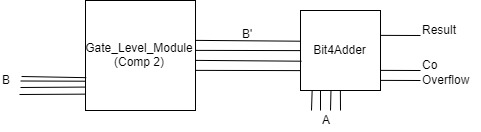
\includegraphics[scale=0.75]{Res4Bit}
\par\end{centering}
\caption{Modulo Res4Bit}

\end{figure}

El dise�o de la ALU esta basado en un operador de 3bits el cual define
que operaci�n y que CCR se muestra a la salida como se vera en el
diagrama l�gico a continuaci�n. Se definieron las siguientes operaciones:

operador=3'b001$\longrightarrow$Suma

operador=3'b010$\longrightarrow$Resta

operador=3'b011$\longrightarrow$ShiftLeft

operador=3'b100$\longrightarrow$Complemento a 2

operador=3'b101$\longrightarrow$Negado

operador=3'b110$\longrightarrow$And

operador=3'b101$\longrightarrow$Or

operador=3'b111$\longrightarrow$Xor

Se definieron las operaciones ShiftLeft, Complemento a 2 y negaci�n
para el primer n�mero ingresado a la ALU. 

\begin{figure}[H]
\begin{centering}
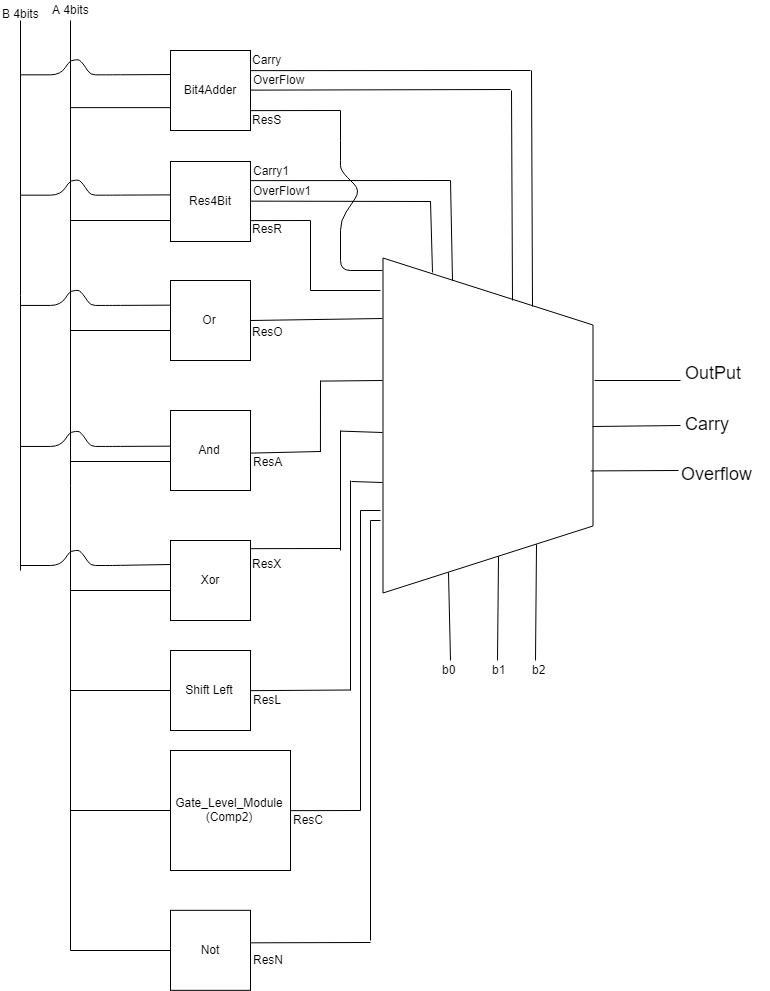
\includegraphics[scale=0.4]{ALU}
\par\end{centering}
\caption{ALU}

\end{figure}

\begin{figure}[H]
\begin{centering}
\begin{tabular}{cccccc}
\toprule 
b0 & b1 & b2 & Output & Carry & Overflow\tabularnewline
\midrule
\midrule 
0 & 0 & 0 & ResS & Carry & Overflow\tabularnewline
\midrule 
0 & 0 & 1 & ResR & Carry1 & Overflow1\tabularnewline
\midrule 
0 & 1 & 0 & ResL & 0 & 0\tabularnewline
\midrule 
0 & 1 & 1 & ResC & 0 & 0\tabularnewline
\midrule 
1 & 0 & 0 & ResN & 0 & 0\tabularnewline
\midrule 
1 & 0 & 1 & ResA & 0 & 0\tabularnewline
\midrule 
1 & 1 & 0 & ResO & 0 & 0\tabularnewline
\midrule 
1 & 1 & 1 & ResX & 0 & 0\tabularnewline
\bottomrule
\end{tabular}\caption{Tabla L�gica de la ALU}
\par\end{centering}
\end{figure}

\end{document}
